%----------------------------------------------------------------------------------------
%	CHAPTER - LITERATURE REVIEW
%----------------------------------------------------------------------------------------

\chapter{Literature Review} % Main chapter title

\label{ChapterLiteratureReview} % Change X to a consecutive number; for referencing this chapter elsewhere, use \ref{ChapterX}

In the literature review chapter, an overview of existing research found in secondary literature, that is relevant to the thesis statement of this paper, is given. Every \gls{srq} is discussed in its own sub-chapter where its relevance to the \gls{mrq} is elaborated. Each sub-chapter ends with a short conclusion and answers to the corresponding research question are given.
Figure \ref{fig:litreviewoverview} shows the correlation between the sub-chapters and the research questions. In chapter \ref{SectionLiteratureReviewSRQ1}, the different methods for user input in virtual reality are analysed The next chapter \ref{SectionLiteratureReviewSRQ2} focuses on existing data interaction patterns in virtual reality. By looking at possible enhancements of existing interaction patterns with new methods for user input, the third SRQ is covered in chapter \ref{SectionLiteratureReviewSRQ3}. To wrap everything up, a conclusion of the literature review is presented in chapter \ref{SectionLiteratureReviewConclusion} which builds the base for the research design in chapter \ref{Research Method}.
\newline
\begin{figure}[h]
	\begin{center}
		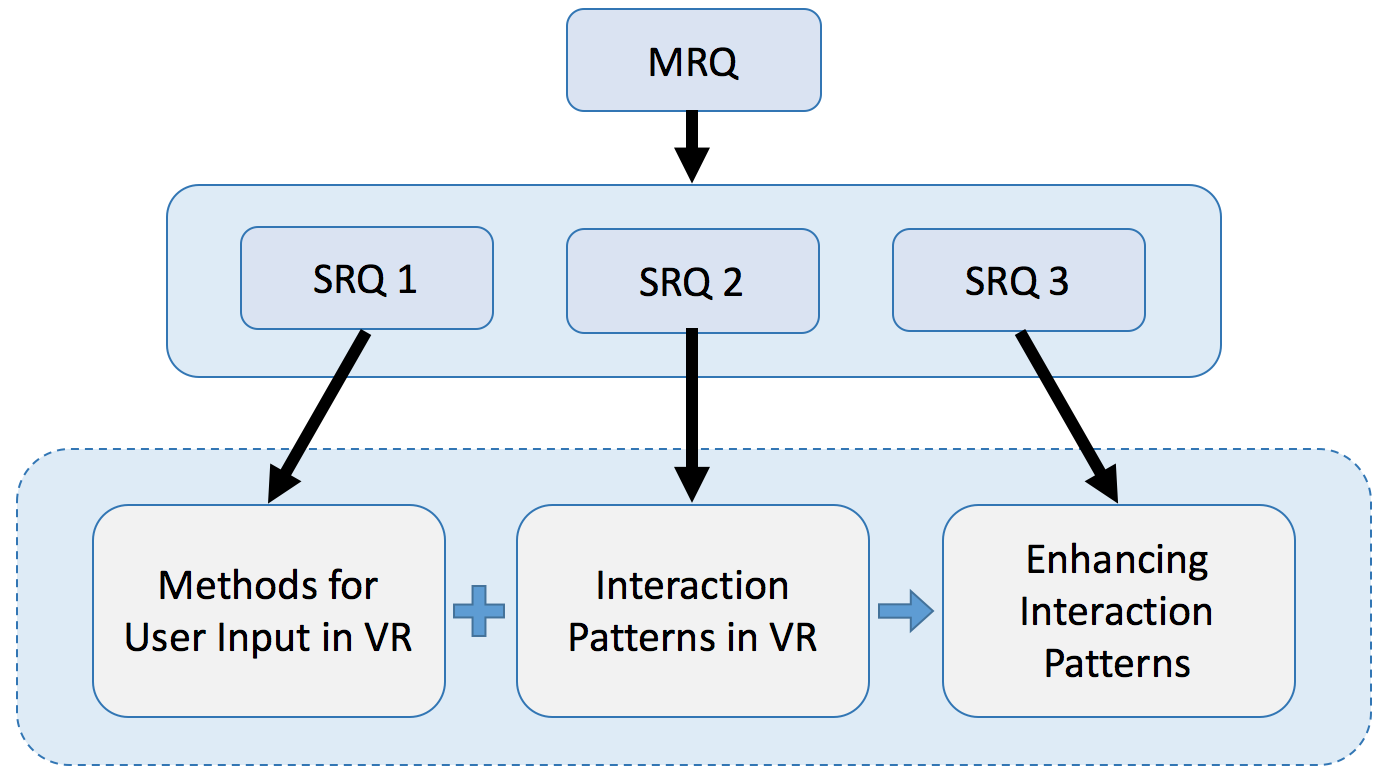
\includegraphics[width=12cm]{03_Figures/05_LitReview/LitReview_SRQ.png}
		\caption[Chapter 2 Overview]{Chapter 2 Overview}
		\label{fig:litreviewoverview}
	\end{center}
\end{figure}

% TODO: ADD FIGURE !!!


%----------------------------------------------------------------------------------------
%	SECTION 1
%----------------------------------------------------------------------------------------

\section{Different Methods for User Input in Virtual Reality}

\label{SectionLiteratureReviewSRQ1}

This chapter deals with the first SRQ, focusing on the currently used and researched different methods for user input in virtual reality. It starts with an introduction and an overview of the different methods while the subsequent chapters give more details on the individual methods.
\begin{framed}
	\textit{SRQ 1: Which methods of user input for virtual reality are researched and what are their advantages and disadvantages?}
\end{framed}

%-----------------------------------
%	SUBSECTION 1
%-----------------------------------
\subsection{Introduction}

\gls{hci} itself has been worked and research on approximately from the 1950s onwards, where the main focus was on the direct manipulation of graphical objects with the mouse as well as gesture recognition \citep{Myers1998}. During this time however, gesture recognition was rather understood as devices that work with pen-based input devices and thus can recognize patterns that are drawn with these pens \citep{Myers1998}. In the regular interaction between human and machines these methods for user input are still fairly sufficient as even today we are still fully relying on having a mouse/track-pad/touch-screen and a keyboard to interact with our computers. \newline
Virtual reality changes this since quite a bit since wearing a \gls{hmd} with its own display obstructs the view on the so far used physical input devices. New solutions had to be found for this changed situation. An overview on the researched interaction patterns with virtual reality is shown in the following sub-chapter


%-----------------------------------
%	SUBSECTION 2
%-----------------------------------

\subsection{Overview of the Different Methods}

The reviewed literature brought up different means in research to interact with the virtual reality environment. In order to review them in a more structured way, they have been grouped based on their core technology (i.e. hand gestures, speech recognition etc.) on which they base on. The regular game controllers have been excluded in this research since they basically are not much different from mouse and keyboard as they do not provide any added interaction functionality.


\subsubsection{Hand Gestures}

\label{SubSubSectionHandGestures}

The by far most utilized and researched interaction method is hand gestures. Since we also heavily rely on this interaction pattern in real life with other human beings, it is fair to assume that the familiarity of it helps the research in a significant way whereas methods that rely on physical hardware often feel more distant. \newline
\cite{Pfeiffer2008} conducted an empirical study about conversational pointing gestures in virtual reality interaction where the focus lied on the system to recognize on which object the user was pointing at. \cite{Pfeiffer2008} distinguished between \gls{ifp} where the direction of where the index finger is pointing at, and \gls{gfp} where an imaginary line between the viewers eye and the tip of the index finger is drawn. Provided the objects are nod too close to each other (>20cm), both methods had equal accuracy and success while tracked with two cameras from different angles and motion capturing \citep{Pfeiffer2008}. Figure \ref{fig:pointinggesture} shows the application of this in an identification game which was part of the empirical study.
\begin{figure}[h]
	\begin{center}
		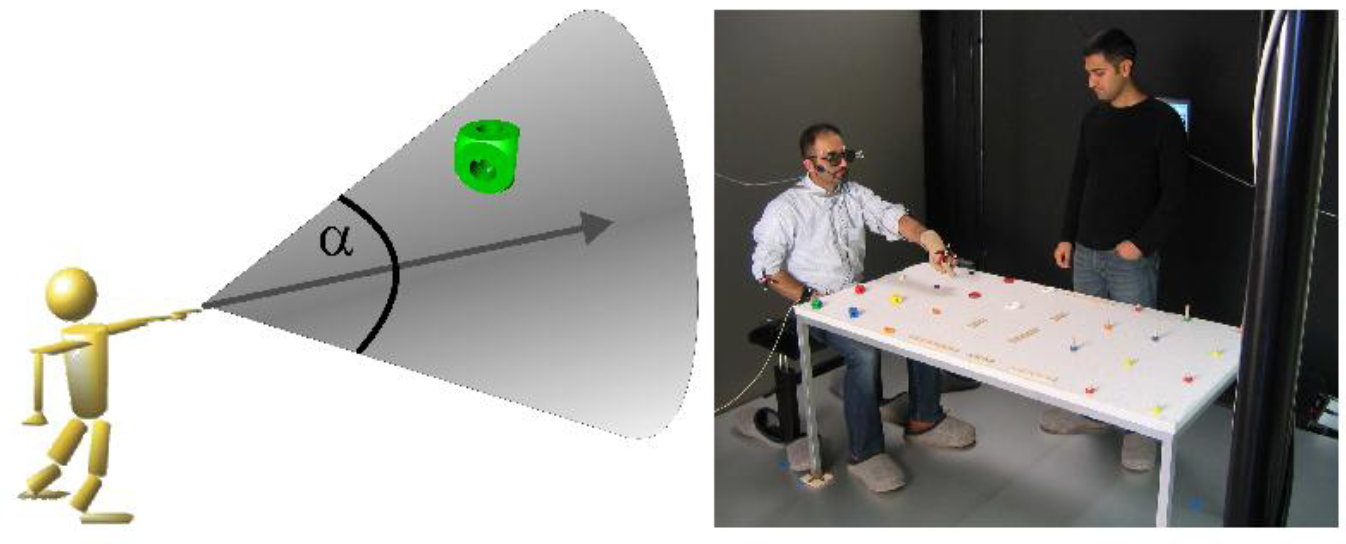
\includegraphics[width=10cm]{03_Figures/05_LitReview/Pfeiffer2008_Pointing.png}
		\caption[Cone-based model for extension of pointing gestures refined for identification game]{Cone-based model for extension of pointing gestures (left) refined for identification game (right) \citep{Pfeiffer2008}}
		\label{fig:pointinggesture}
	\end{center}
\end{figure}
\newline
A similar approach has been research by \cite{Rautaray2011} who used a single camera with an application that did the image capturing, locating the hand and its orientation and finally model the gesture to find a match for predefined gestures. The focus relied on simple gestures for \textit{punch} (three fingers), \textit{grab} (fist), \textit{throw} (five fingers), and to \textit{move forward} (thumb up) within a simple VR game \citep{Rautaray2011}. The recognition rate was between 80\% and 94\% (depending on the gesture), which might not be accurate enough for practical use cases as also acknowledged by \cite{Rautaray2011}. \newline
In a more recent study of \cite{Khundam2015}, it was not cameras that were used to track the hand gestures but a Leap Motion (an in-air controller) attached to the front of an Oculus Rift. Figure \ref{fig:leapmotion} shows the different gestures that were implemented by \cite{Khundam2015} in order to navigate within a virtual environment. Depending on how far the hand is moved towards a certain angle, the speed of the movement can be influenced to increase or decrease it \citep{Khundam2015}. Although the applied gestures are understandable and easy to learn, they still brings some unfamiliarity with them since in real life movement already has a specific gesture which however utilizes the legs and not the hands.
\begin{figure}[h]
	\begin{center}
		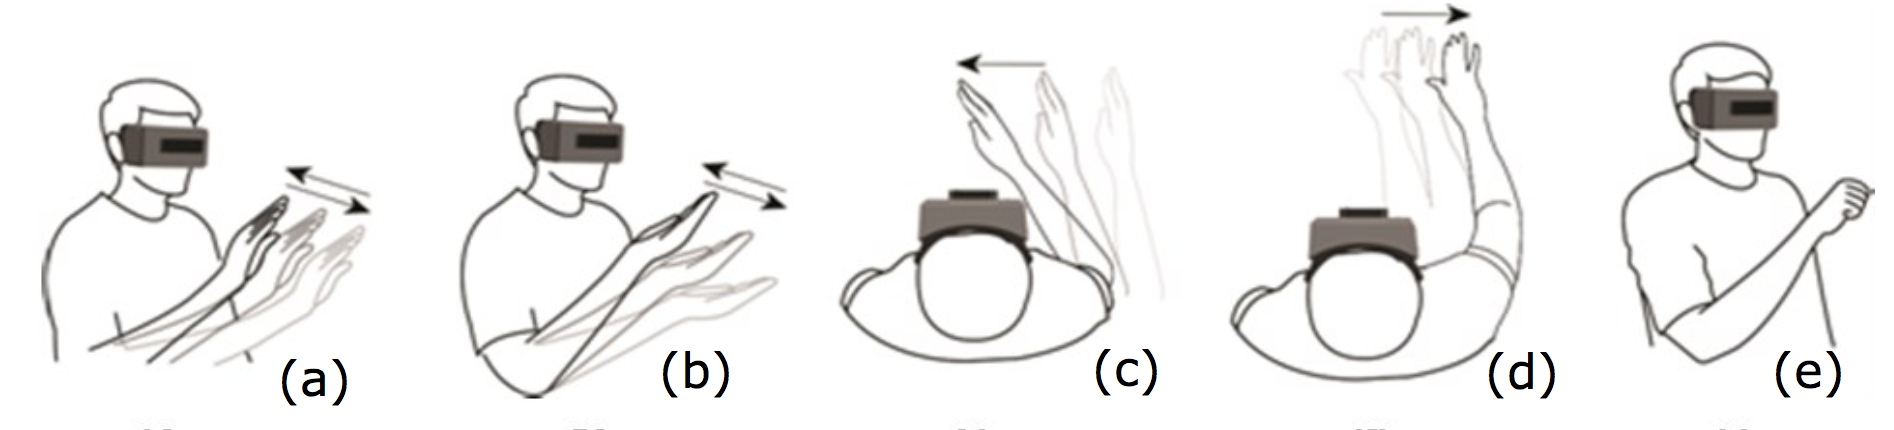
\includegraphics[width=14cm]{03_Figures/05_LitReview/Khundam2015_LeapMotion.png}
		\caption[Hand gestures for forward/backward movement, stepping left/right and holding position]{Hand gestures for forward/backward movement (a,b), stepping left/right (c,d) and holding position (e) \citep{Khundam2015}}
		\label{fig:leapmotion}
	\end{center}
\end{figure}
\newline
For their research on static and stroke gestures, \cite{Chun2015} made use of a depth-camera in order to track hand gestures and combined it with speech recognition. The latter is discussed in more detail in chapter \ref{SubSubSectionSpeechRecognition} which covers the methods of speech recognition in general. \cite{Chun2015} defined different hand and finger gestures for selecting, moving, scaling, rotating, copying and deleting objects, all of which actions had to be confirmed by a specific yes/no gesture. This set of gestures makes it a very natural, intuitive and interactive way for the user to alter virtual objects. As often with the use cameras, there are limitations to it. The hand has to be tracked properly for the whole performance of the gesture and it has to be done with the right speed for a proper recognition of the command \citep{Chun2015}.


\subsubsection{Gesture Controllers}

Very similar to the hand gestures, the gesture controllers intend to improve the tracking of the hand movements by adding hardware to the hands of the users that is easier to track but still leaves options for simple interaction with buttons and triggers. \newline
One of the first commercial gesture controllers was the \textit{PlayStation Move}, introduced by \cite{Sony2010}. While the controller itself can detect its own motion, the position is tracked with a camera attached to the PlayStation. This allows for a more accurate tracking of a specific point which \cite{Takala2014} made use of by attaching a PlayStation Move to their HMD in order to have a more accurate positioning than it was possible with solely the Microsoft Kinect. \newline
Alongside the \textit{HTC Vive} HMD, a new gesture controller also have been introduced \citep{Htcvive2016}. In combination with the Lighthouse technology (described in chapter \ref{360MotionTracking}), the controllers can also be properly tracked if they are e.g. hidden behind the back of the user, which is not possible with the PlayStation Move. Figure \ref{fig:gesturecontroller} shows this controller with its unique design for the tracking sensors (6) and a combination of track-pad (2), buttons (1, 3 and 8) and a trigger (7). By putting the thumb on the track-pad, the index finger on the trigger and the other three fingers on the side button it almost allows to track the grabbing motion of the hand.
\begin{figure}[h]
	\begin{center}
		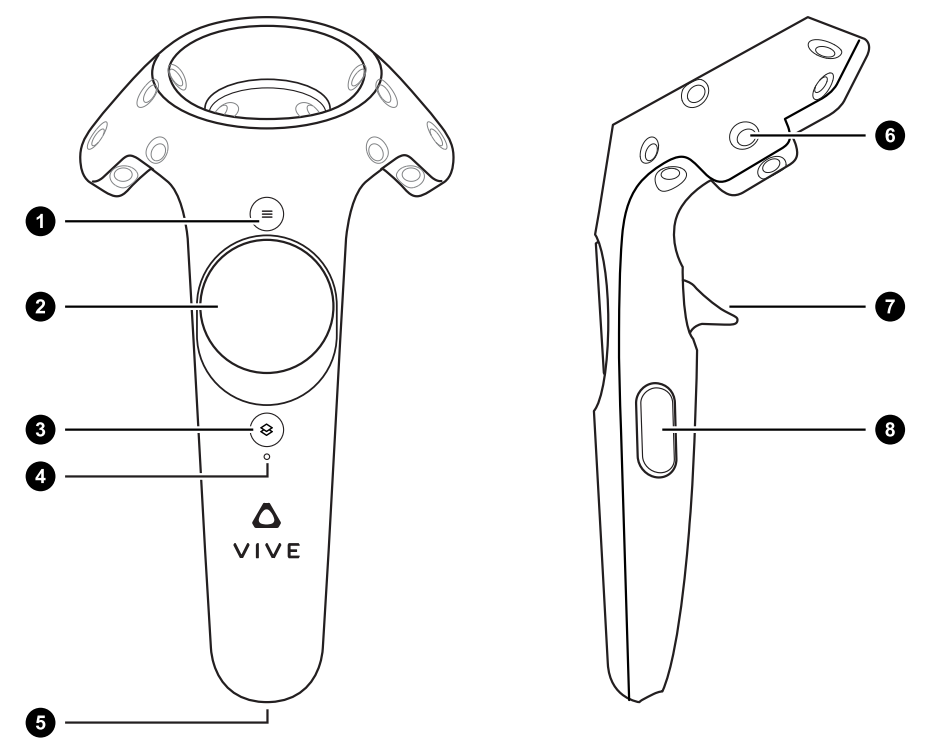
\includegraphics[width=10cm]{03_Figures/05_LitReview/HTCCorp2016_GestureController.png}
		\caption[Gesture Controller for the HTC Vive]{Gesture Controller for the HTC Vive \citep{HTCCorp2016}}
		\label{fig:gesturecontroller}
	\end{center}
\end{figure}


\subsubsection{Speech Recognition}

\label{SubSubSectionSpeechRecognition}

The second natural interaction after hand gestures is speech recognition It is often combined with hand gesture as they can complement each other quite seamlessly. \newline
For the navigation within 3D scans from \gls{mri} or \gls{ct}, \cite{Muller1998} proposed a speech recognition system as illustrated with an example in figure \ref{fig:speechrecognitionmedical}. With semantic decoding and a semantic structure, the commands can be interpreted and processed by the intention decoder to tell the system what to \citep{Muller1998}. This is a very time-consuming process since all commands have to be prepared and acoustic-phonetic models need to be generated during the collection of training data. Provided the users followed the instructions, a 99.8\% semantic accuracy could be achieved which basically means that the system is almost fully accurate in this scenario \citep{Muller1998}.
\begin{figure}[h]
	\begin{center}
		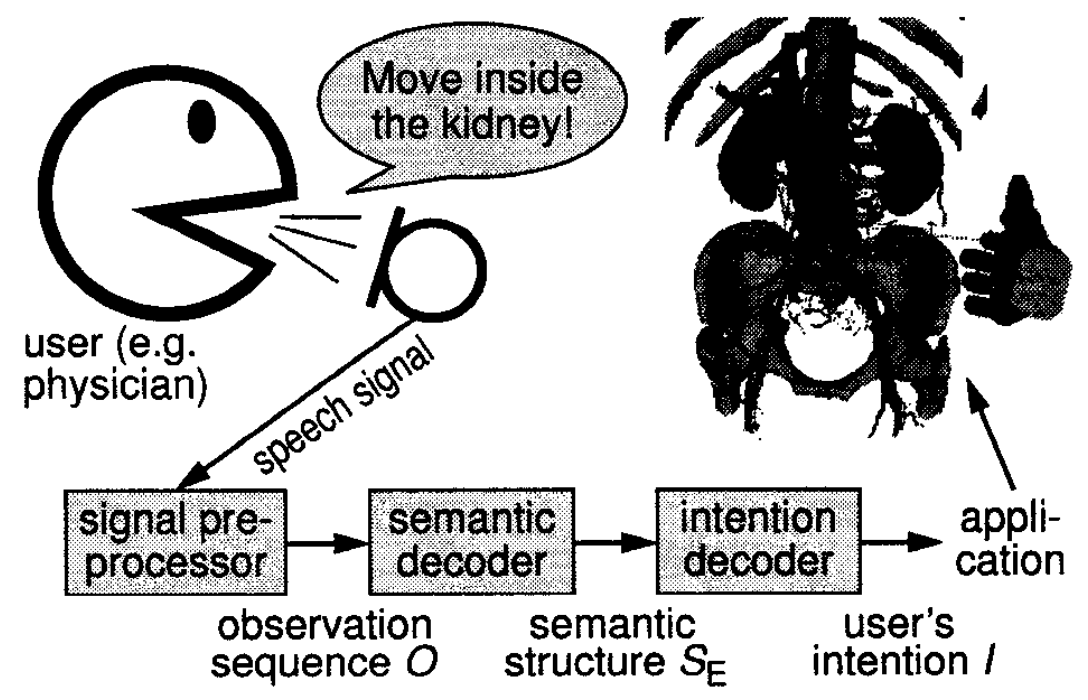
\includegraphics[width=10cm]{03_Figures/05_LitReview/Muller1998_SpeechRecognition.png}
		\caption[Architecture and example of speech recognition and interaction for physicians]{Architecture and example of speech recognition and interaction for physicians \citep{Muller1998}}
		\label{fig:speechrecognitionmedical}
	\end{center}
\end{figure}
\newline
\cite{Uchino2008} combined speech recognition with a camera to identify where the user is pointing at on a computer screen to interact with a virtual agent. In their example, a set of pens with different colours are presented to the user where the selection is made in combination with gestures (pointing at the pen) and speech (e.g. "\textit{Please give the red one}") \citep{Uchino2008}. Figure \ref{fig:speechrecignitionpen} shows how such a conversation with a virtual agent can proceed where the agent picks the wrong pen based on the pointing and ambiguous speech and thus has to be corrected to pick the one with the right colour Although this research was not focussed on virtual reality, this research can also be applied in virtual reality which might even improve the accuracy of the pointing gesture.
\begin{figure}[h]
	\begin{center}
		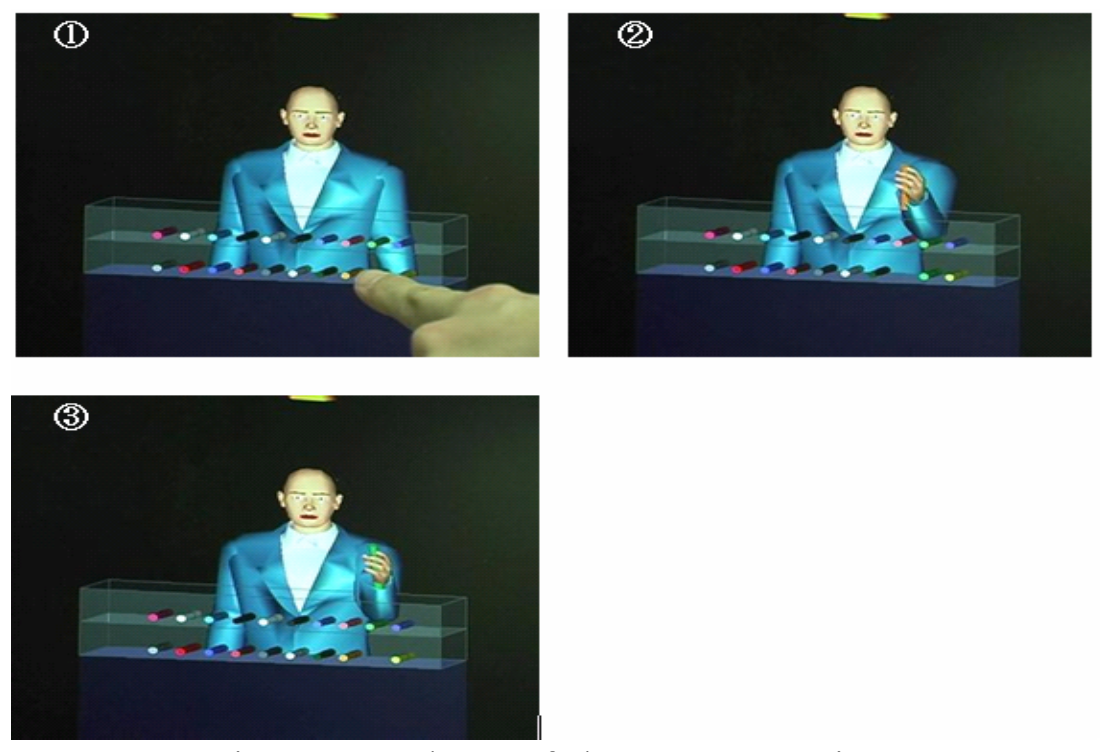
\includegraphics[width=10cm]{03_Figures/05_LitReview/Uchino2008_SpeechPointing.png}
		\caption[Flow of a conversation with the virtual pen agent]{Flow of a conversation with the virtual pen agent \citep{Uchino2008}}
		\label{fig:speechrecignitionpen}
	\end{center}
\end{figure}
\newline
As described in chapter \ref{SubSubSectionHandGestures}, \cite{Chun2015} utilized hand gestures to interact with virtual objects and further enhanced them with speech recognition. While objects can be altered in their spatial appearance, speech is used to change the colour of the object or ask questions about the type, shape or colour of it \citep{Chun2015}. Instead of relying on a physical device with buttons to change the colours, a multi-modal interaction combines speech and gesture to a more natural and intuitive method that is also closer to the real world \citep{Chun2015} .


\subsubsection{Physical Placement of Interactive Objects}

Quite a bit older, from the 1990s, is the idea of dynamically placing physical knobs and switches in front of a seated user wearing a HMD \citep{Latham1997}. The trajectory of the users hand and its movement is extrapolated in order to move the correct type of control in the right position just when it is expected in the virtual reality environment \citep{Latham1997}. Figure \ref{fig:touchcockpit} shows the concept of \cite{Latham1997} as well as how the final design looked like. Since such a machine requires a lot of time to design and build, it can be assumed that these are parts of the reason why not many further advancements were undertaken.
\begin{figure}[h]
	\begin{center}
		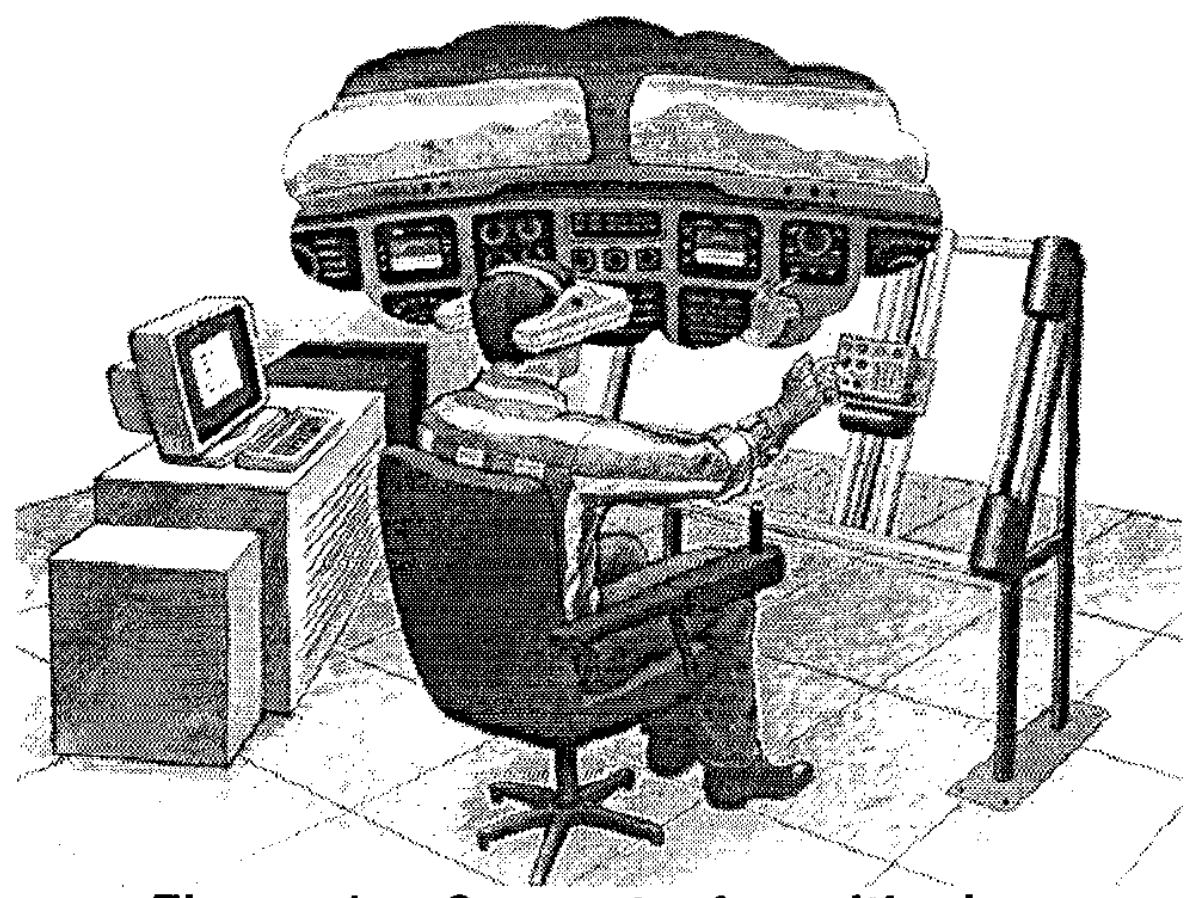
\includegraphics[width=6cm]{03_Figures/05_LitReview/Latham1997_Concept.png}
		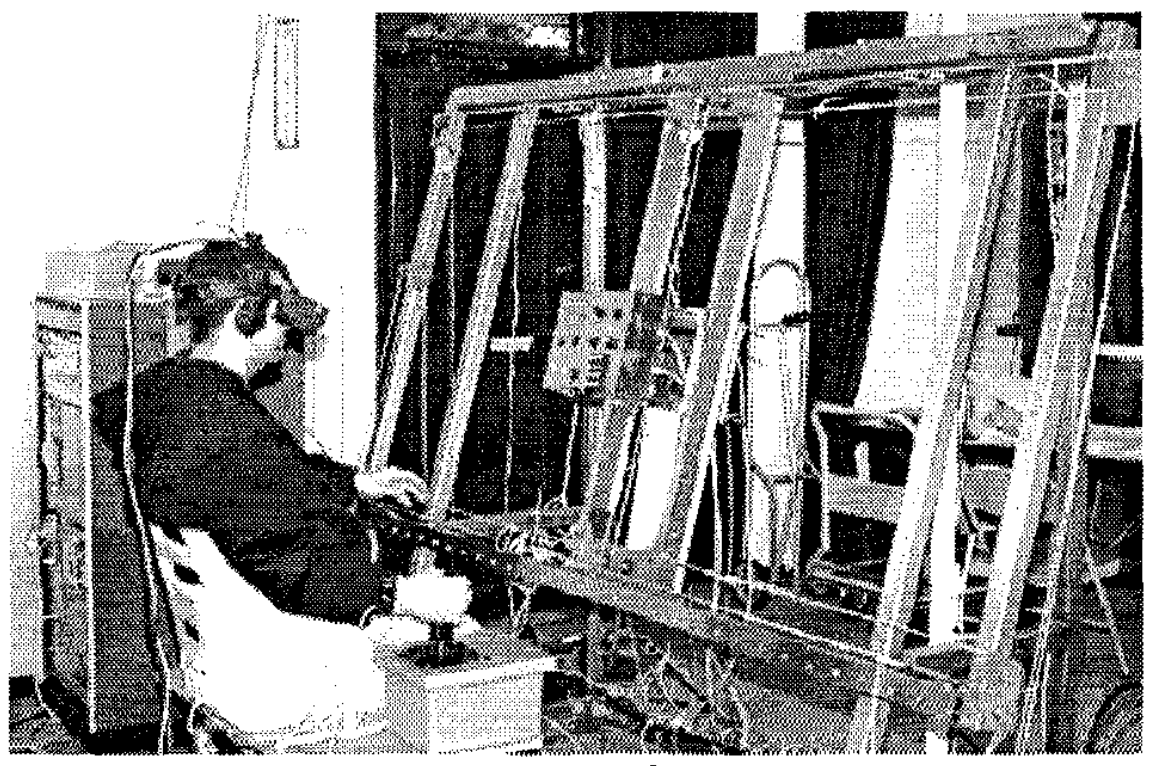
\includegraphics[width=7cm]{03_Figures/05_LitReview/Latham1997_FinalDesign.png}
		\caption[Concept and final design of positioning instrument controls to be touched in a virtual cockpit]{Concept (left) and final design (right) of positioning instrument controls to be touched in a virtual cockpit \citep{Latham1997}}
		\label{fig:touchcockpit}
	\end{center}
\end{figure}


\subsubsection{Full Body Tracking}

In June 2010, Microsoft announced the \textit{Kinect for Xbox 360}, a controller-free gaming device for the living room \citep{Microsoft2010}. Instead of relying on any physical input devices, the Kinect contains a camera with motion-sensing technology that can track up to 48 points of movement on the human body, turning the player himself into a controller \citep{Microsoft2010}. \newline
Based on this technology, \cite{Takala2014} proposed a combination of a full body avatar controlled by Kinect with the Oculus Rift as display. This combination proved to be quite powerful although they were facing a couple of challenges as well. The Kinect sometimes lost track of the hands or the movement was not recognized at all which \cite{Takala2014} tried to resolve by attaching a PlayStation Move to the HMD and put a Razer Hydra controller into the hands (Figure \ref{fig:kinectbody}). Although this improved the situation, different latencies of the individual dampened the experience. Furthermore, although Kinect was used for full-body tracking, only the movement of the hands and legs was utilized, whereas the movement within the virtual world was still relying on a physical controller.
\begin{figure}[h]
	\begin{center}
		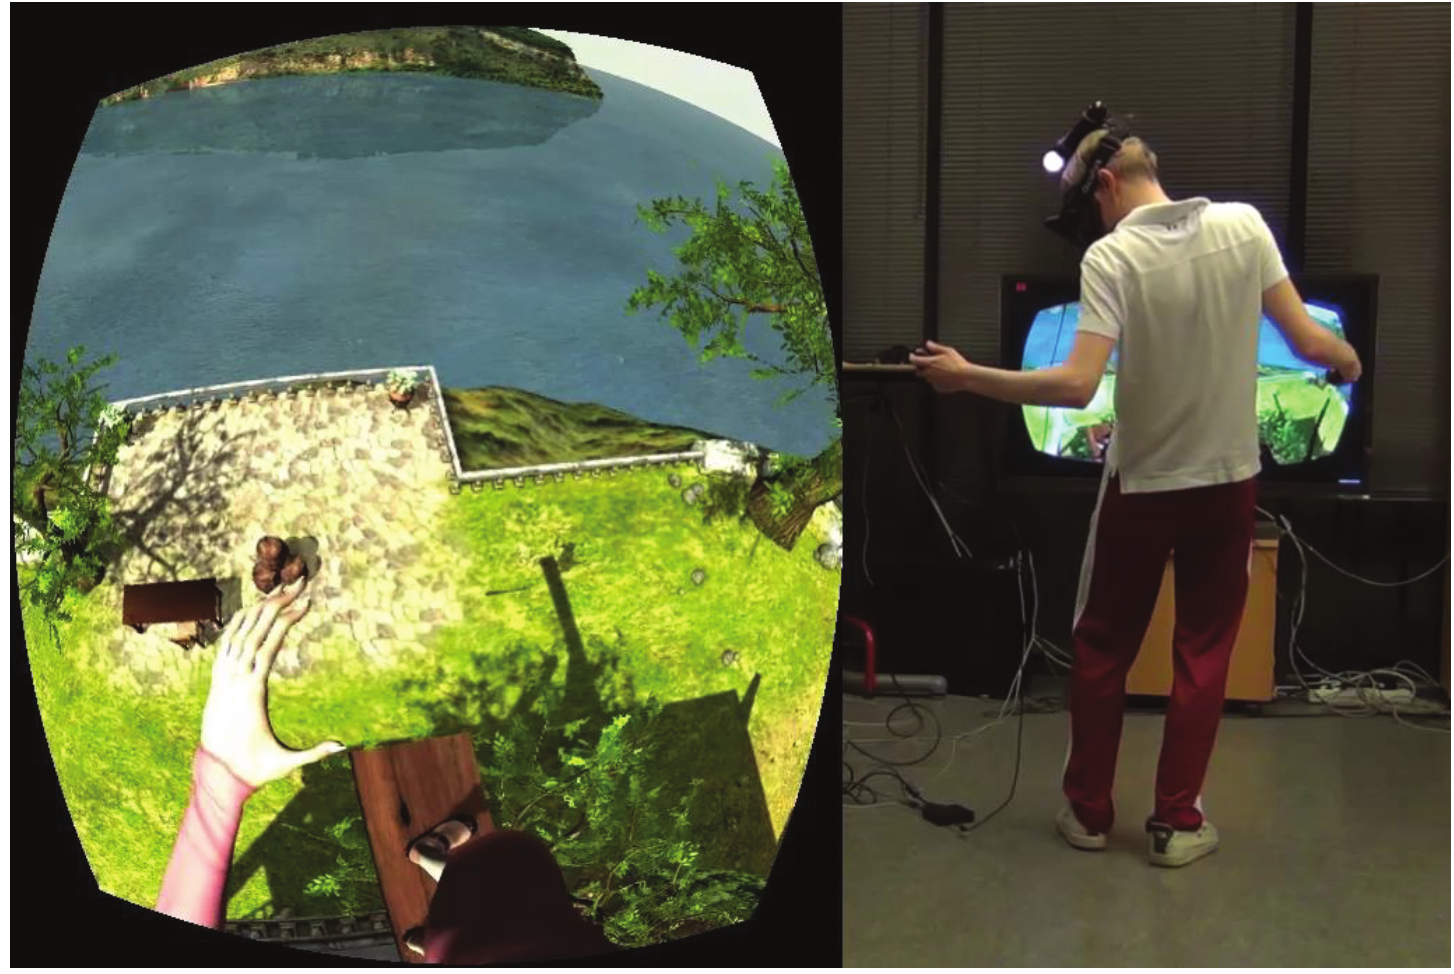
\includegraphics[width=12cm]{03_Figures/05_LitReview/Takala2014_KinectBody.png}
		\caption[Player's view of their virtual body that is tracked with Kinect]{Player's view of their virtual body (left) that is tracked with Kinect (right) \citep{Takala2014}}
		\label{fig:kinectbody}
	\end{center}
\end{figure}


\subsubsection{360° Motion Tracking}
\label{360MotionTracking}

One of the latest additions to the interaction possibilities is the 360° motion tracking, introduced with the HTC Vive which was just released in April 2016 \citep{Htcvive2016}. Figure \ref{fig:lighthouses} shows the setup of the two base stations (i.e. Lighthouses) in opposing corners of the room that will be used for the 360° motion tracking. In essence, the two Lighthouse base stations emit a laser sweep across the room 60 times a second with a flash in between which allows any device with photo-sensors to calculate its exact position relative to the base station(s) \citep{Gizmodo2015}. This allows for a very accurate tracking and due to the opposing corners, at least one Lighthouse always has direct \textit{line of sight} to the HMD and the controllers. \newline
With this additional sensor information, the movement of the HMD and the controllers is tracked in all three axis and allow for new movements to be recognized, such as crouching or jumping within the relations of the room.
\begin{figure}[h]
	\begin{center}
		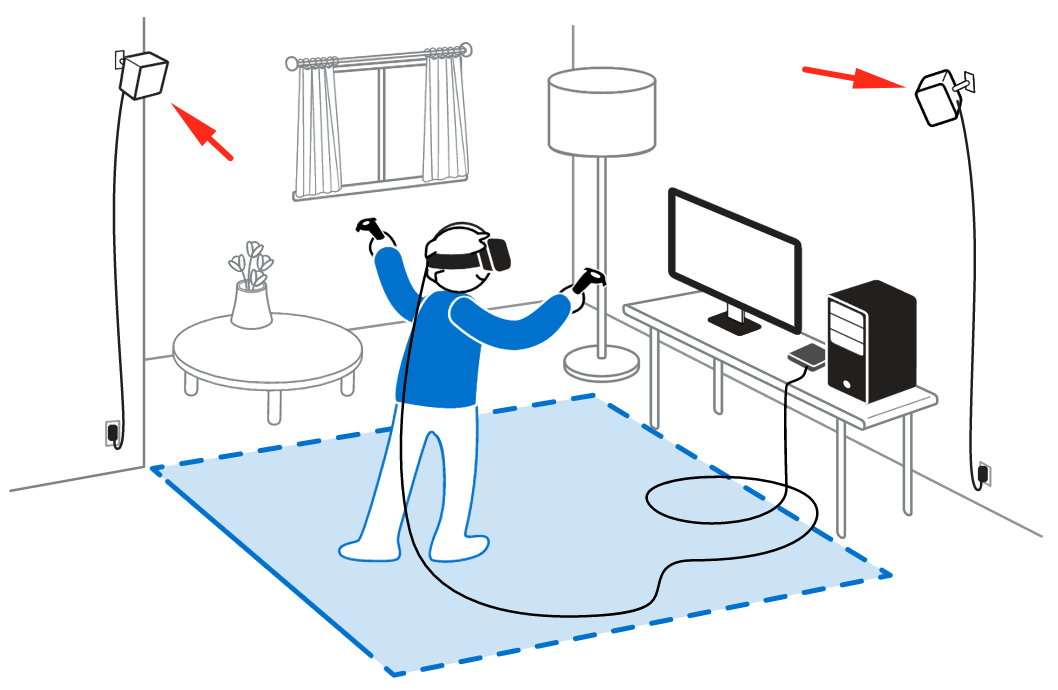
\includegraphics[width=10cm]{03_Figures/05_LitReview/HTCCorp2016_LighthouseRoomScale.png}
		\caption[Two Lighthouse in opposing corners allow for 360° motion tracking]{Two Lighthouse in opposing corners allow for 360° motion tracking \citep{HTCCorp2016}}
		\label{fig:lighthouses}
	\end{center}
\end{figure} \newline
A more simplified variation of this is described by \cite{Donalek2014}, who used a ViconTM motion-capturing system with infrared markers on the HMD to track its spatial location. This allowed \cite{Donalek2014} to also recognize movements such as kneeling down or looking over and around objects in the scene, however always limited by the volume that was covered by the Vicon system.


%-----------------------------------
%	SUBSECTION 3
%-----------------------------------

\subsection{Conclusion}

\begin{table}[b]
	\begin{center}
		\begin{tabular}{ | p{3.7cm} | p{4.9cm} | p{4.9cm} | } 
			\hline
			\textbf{Method} & \textbf{Advantages} & \textbf{Disadvantages} \\
			\hline
			Hand Gestures & 
			- Highest familiarity \newline - Inexpensive & 
			- Limited tracking area \newline - Only from one angle \newline - Decreasing accuracy with faster movement  \\
			\hline
			Gesture Controllers &
			- Very accurate \newline - Similarity to hand gestures \newline - Buttons for more interaction &
			- Additional device required \newline - Have to be held all the time \\
			\hline
			Speech Recognition &
			- Most natural to humans \newline - Known from smartphones &
			- Different languages, dialects \newline - Requires silent area \\ 
			\hline
			Physical Placement of Objects &
			- Realistic experience \newline - Tangible interaction with VR &
			- Expensive \newline - Difficult to build \newline - Stationary \\ 
			\hline
			Full Body Tracking &
			- Tracks all extremities \newline - Natural interaction possible &
			- Only from one angle \newline - Limited accuracy on details \\ 
			\hline
			360° Motion Tracking &
			- Room-scale movement \newline - Very accurate \newline - Spatial positioning on all three axis &
			- Only dedicated HMD and controllers can be tracked \newline - Stationary (base stations) \\ 
			\hline
		\end{tabular}
		\caption{Advantages and disadvantages/limitations of different methods for user input in virtual reality}
		\label{tbl:methodscomparison}
	\end{center}
\end{table}

The literature review on different methods for user input in virtual reality showed that there are various types can be used or even combined. \newline
There are six main methods for user input in virtual reality. These are hand gestures, gesture controllers, speech recognition, physical placement of interactive objects, full body tracking and 360° motion tracking. Hand gestures track the movement of the whole hand and/or the individual fingers with one or more (regular, infra-red or depth) cameras. Gesture controllers are physical devices with buttons that are held in the hands and also tracked in their spatial position. Speech recognition tries to understand and interpret spoken words and sentences in order to find the correct commands. The physical placement of interstice objects extrapolates the movement of the hand to physically place a button in front of the finger where a virtual one is shown in V Full body tracking uses cameras to track the whole body including the movement of all extremities from one angle. Finally, 360° motion tracking can locate the position of special devices within an actual room on all three axis from opposing corners. The most used method in the reviewed literature is the hand gestures, followed by the hand gestures in combination with speech recognition \newline
Depending on the chosen method, there are advantages and disadvantages (or even limitations) for certain use cases. Table \ref{tbl:methodscomparison} shows a summary of these findings.

In regards of the thesis statement, a combination of two methods is recommended to outweigh the individual disadvantages and utilize the benefits of both methods.


%----------------------------------------------------------------------------------------
%	SECTION 2
%----------------------------------------------------------------------------------------

\section{Existing Interaction Patterns in Virtual Reality}

\label{SectionLiteratureReviewSRQ2}

This chapter addresses the second SRQ by having a look at existing interaction patterns in virtual reality and evaluating their strengths and weaknesses. It starts with a short introduction, followed by an analysis of the visual information seeking mantra and the idea of multi-modal interaction. Then more details are given on different interaction patterns for navigation, selection and manipulation, before the importance of immersion and task performance is elaborated. A conclusion summarises the research done in this chapter.
\begin{framed}
	\textit{SRQ 2: Which ways of interaction with multi-dimensional data exist and what are their strengths and weaknesses?}
\end{framed}

%-----------------------------------
%	SUBSECTION 1
%-----------------------------------

\subsection{Introduction}

During the 1960s, the first interaction patterns such as clicking or grabbing and moving objects have been defined on which even now we are still relying on with mouse and keyboard \citep{Myers1998}. But with wearing a \gls{hmd}, the situation changes as it obstructs our view on the so well known devices. New methods for user input had to be research and inherently also new interaction patterns had to be defined. \cite{Donalek2014} mentioned that a new tool is required where physical gestures can be used to manipulate with virtual objects. In order to understand what kind of gestures should be considered, the Visual Information Seeking Mantra of \cite{Shneiderman1996} is looked at.


%-----------------------------------
%	SUBSECTION 2
%-----------------------------------

\subsection{Visual Information Seeking Mantra}

\cite{Shneiderman2005} defined principles for direct manipulation, including:
\begin{itemize}[noitemsep,nolistsep]
	\item visual representation of the world of action including both the objects and actions
	\item rapid, incremental and reversible actions
	\item selection by pointing(instead of typing)
\end{itemize}
Based on this, \cite{Ahlberg1994} proposed the Visual Information Seeking Principle in 1994 that focused in displaying a graph with buttons and sliders for real-time manipulation of the displayed data. This concept fulfilled all principles for direct manipulation and was so successful that it became the foundation for the Visual Information Seeking Mantra \citep{Shneiderman1996}. \cite{Shneiderman1996} was looking at many visual design guidelines but fundamentally always concluded the following mantra:
\begin{framed}
	\textit{Overview first, zoom and filter, then details-on-demand}
\end{framed}
As an abstraction of reality, \cite{Shneiderman1996} further defined seven tasks that are inherently crucial for the work with data:
\begin{itemize}[noitemsep,nolistsep]
	\item Overview \textit{(Gain an overview of the entire collection)}
	\item Zoom \textit{(Zoom in on items of interest)}
	\item Filter \textit{(Filter out uninteresting items)}
	\item Details-on-demand \textit{(Select and item or group and get details when needed)}
	\item Relate \textit{(View relationships among items)}
	\item History \textit{(Keep a history of actions to support undo, replace and progressive refinement)}
	\item Extract \textit{(Allow extraction of sub-collections and of the query parameters)}
\end{itemize}



Visual Information Seeking: Tight Coupling of Dynamic Query Filters with Starfield Displays \cite{Ahlberg1994}

The Eyes Have It: A Task by Data Type Taxonomy for Information Visualizations \cite{Shneiderman1996}

Beyond Guidelines: What Can We Learn from the Visual Information Seeking Mantra? \cite{Craft2005}

When the visual information-seeking mantra fails \cite{Neil2006}

A review and extension of the Visual Information Seeking Mantra (VISM) \cite{Stauffer2016}


%-----------------------------------
%	SUBSECTION 3
%-----------------------------------

\subsection{Multi-modal Interaction}

\cite{Bunt1998} stated that "Human communication is inherently multimodal in nature".

One approach to the problems of understanding natural language is to enable multiple communication modes. In a multimodal  user interface, a user might make a spoken natural language request, but supplement it with one or more gestures. For example, the user might say "Put that there," while also point- ing with the hand or pressing a button (Bolt 1980).  \cite{Rosson2002}


%-----------------------------------
%	SUBSECTION 4
%-----------------------------------

\subsection{Interaction Patterns}


%-----------------------------------
%	SUBSUBSECTION 1
%-----------------------------------

\subsubsection{Navigation}

Since the user loses all sight of their hands from within the device, traditional mouse and keyboard in- teraction is limited. While we do not address specific interaction challenges here, we did want to avail ourselves of the head tracking capabilities of the HMD. Since the device tracks the position and direction of the camera, we can also utilize this information to de- termine what the user is looking at, use this information to identify focal points, aid the user in making selections, and provide instan- taneous details of the selected data. \cite{Kwon2015}

An example of this is the ability to track the users head position so that we can appear to look around object, this is how as humans we are familiar with examining objects of interest, rather than moving a mouse. In a totally immersive virtual environment we can use body movement to walk around objects or put our head inside virtual representation of our data. Also within an immersive environment it is possi- ble to map the users hand position in the real world to a virtual hand in the VE, therefore allowing the user to manipulate virtual objects. \cite{Jamieson2007}


In our virtual environment, a fully immersed person is working on a specific task and several (up to 20) outsiders (participants) observe the fully immersed person and would like to comment and affect the fully immersed person’s work. \cite{Deligiannidis2003}

The current communication technique used is vocal instruction, which is distracting to everyone. This paper presents a technique in which the fully immersed person and the participants can interact using a second camera directed for a third person’s view of the environment. This technique attempts to provide the best of both worlds (first and third person views) so the formerly passive participants can become more immersed in the environment. \cite{Deligiannidis2003}

The space around the participant who is controlling the camera is divided into two hemispheres, the top and the bottom one. Camera manipulation is activated when both sensors enter the top hemisphere, and hand manipulation is activated when both hands enter the bottom hemisphere. \cite{Deligiannidis2003}


At our demonstrations, we observed that many users had difficulty interacting with keyboard and mouse when they could not see their hands, but most users were able to use the Xbox controller intuitively. Users were able to “fly” through the data and, using the Oculus head-tracking, look around and view the data from different perspectives. \cite{Drouhard2015}


%-----------------------------------
%	SUBSUBSECTION 2
%-----------------------------------

\subsubsection{Selection}

PS Move or Razer Hydra controller is used to control locomotion, and for selecting and manipulating objects. \cite{Takala2014}


Simple selection techniques (a) Ray-based selection is effected by choosing first object to intersect the ray from the hand (Object A in this case) (b) Small Volume Selection is effected by choosing ever object’s volumes intersect the volume attached to the hand (Object C). (c) Cone Selection can be effected by choosing all objects that lie within the cone (Objects E and F). \citep{Steed2006}

\begin{figure}[h]
	\begin{center}
		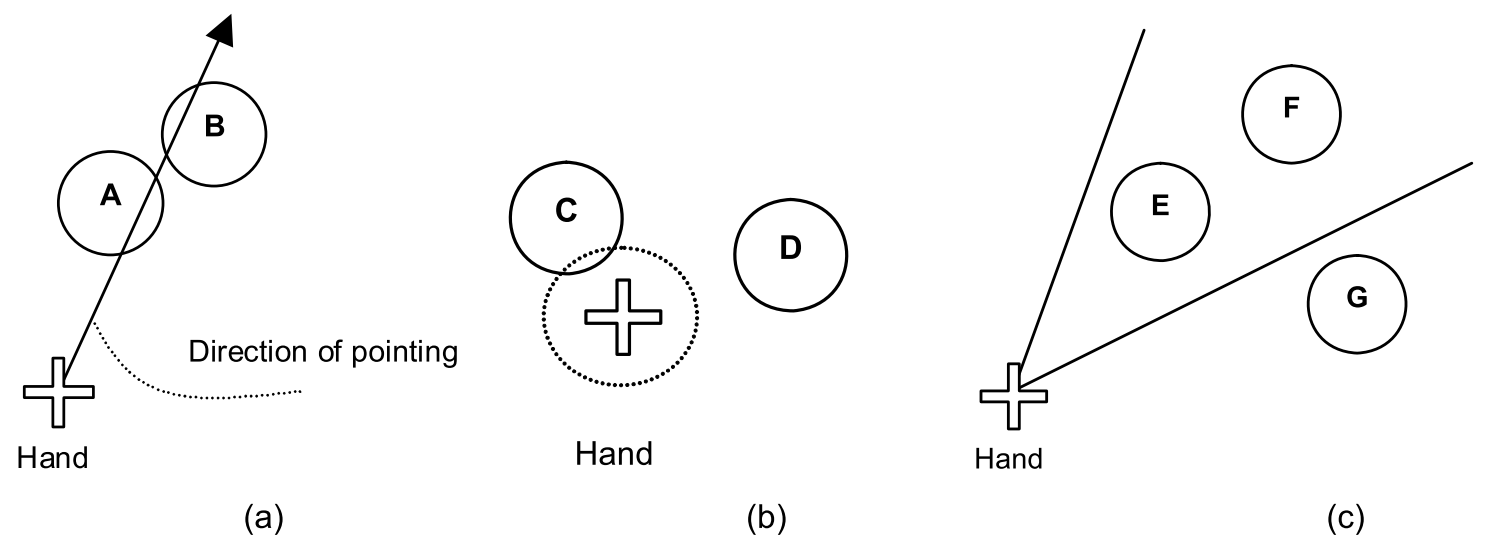
\includegraphics[width=14cm]{03_Figures/05_LitReview/Steed2006_SelectionTechniques.png}
		\caption[tbd]{tbd \citep{Steed2006}}
		\label{fig:selectiontechniques}
	\end{center}
\end{figure}


Since the user loses all sight of their hands from within the device, traditional mouse and keyboard in- teraction is limited. While we do not address specific interaction challenges here, we did want to avail ourselves of the head tracking capabilities of the HMD. Since the device tracks the position and direction of the camera, we can also utilize this information to de- termine what the user is looking at, use this information to identify focal points, aid the user in making selections, and provide instan- taneous details of the selected data. \cite{Kwon2015}


When the user uses this reticle to select a node, the node and all its neighbors are brought closer to the user’s viewpoint. Similarly, all the control points for all affected edges are also brought closer. This serves to separate the selected node and its neighbors from the rest of the graph and bring them into a closer, focal plane. To further accentuate this, we apply a halo technique to the selected node’s edges. The overall effect is that the selection is easily distinguished from the remainder of the graph, and the immediate connections are easy to visually follow to their destinations. Multiple nodes can be selected and brought into this focal plane, allowing the user to explore any potentially interesting paths or relations that they find. \cite{Kwon2015}


Our immersive visualization also incorporates gaze interaction, arguably the most natural form of interaction in virtual reality environments. In order to help users target objects more effectively, we provide a crosshair reticle that is rendered visible when a button is pressed to enter “target mode.” If, when the trigger button is pressed, the reticle is targeting a data object, the trigger also bookmarks that data object and highlights it in a contrast color. When the trigger button is pressed, the user’s location is saved regardless of whether or not a data object is bookmarked \cite{Drouhard2015}


Interactive brushing of a 3D scatterplot inside a CAVE-like virtual environment. The brushing operation begins with an empty selection box (left). The user then specifies the selection box’s body diagonal by moving the input device. This locally highlights points in the selection in real-time (center). Only after releasing the input device’s button, the update is remotely computed and the selection for all plots is shown (right). \citep{Hentschel2009}
\begin{figure}[h]
	\begin{center}
		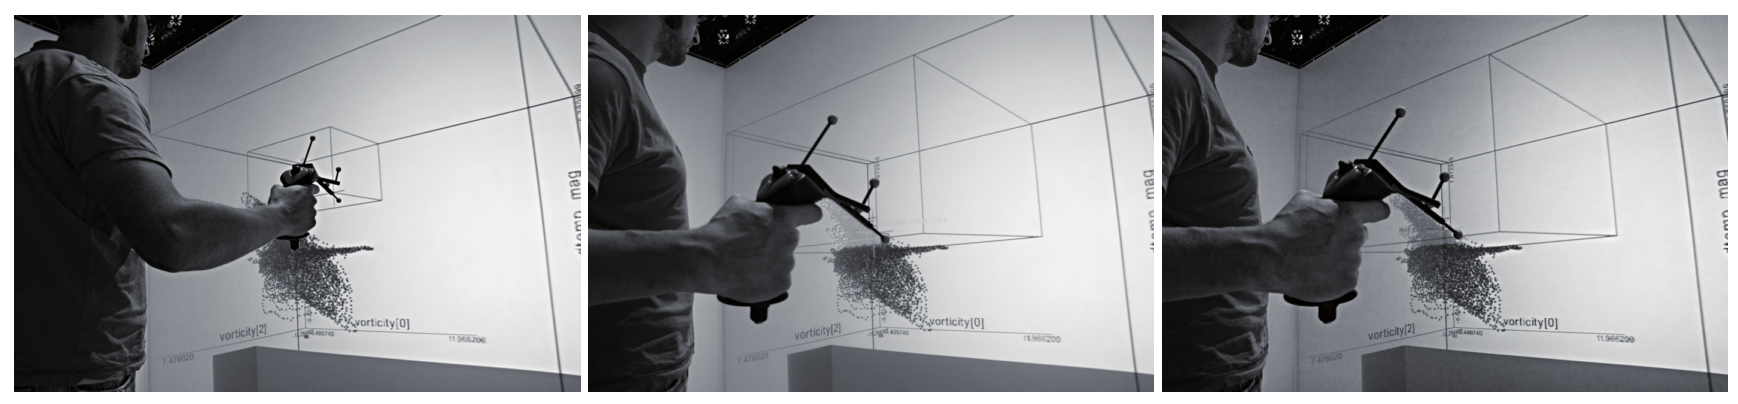
\includegraphics[width=14cm]{03_Figures/05_LitReview/Hentschel2009_InteractiveBrushing.png}
		\caption[tbd]{tbd \citep{Hentschel2009}}
		\label{fig:interactivebrushing}
	\end{center}
\end{figure}


%-----------------------------------
%	SUBSUBSECTION 3
%-----------------------------------

\subsubsection{Manipulation}

As early as in the 1980s, interaction patterns with data have already been defined, such as the "Put-That-There" voice and gesture interface as described by \cite{Bolt1980}. This interfaces focus on certain voice command to manipulate objects in a virtual space which have been defined as following \citep{Bolt1980}:
\begin{itemize}[noitemsep,nolistsep]
	\item "Create..." \textit{(a default object, with default size and colour on a default position)}
	\item "Move..." \textit{(an object to a specific position)}
	\item "Make that..." \textit{(altering an object in colour and size)}
	\item "Delete..." \textit{(removal of an object)}
	\item "Call that..." \textit{(give an object a name to which it can be referred to)}
\end{itemize}
In addition, the spoken \textit{"there"} serves as some kind of voice button where the \textit{"there"} refers to the cursor position, thus introducing the gestures as an input method for this interface \citep{Bolt1980}. \newline
It can be seen that even more than three decades ago, the need to simplify more complicated interactions such as changing the colour of an object which would require multiple inputs with mouse/keyboard, were tested to be simplified with new means of interaction patterns.


Since wearing of the goggles effectively precludes the use of a keyboard interface, we need a tool where a user can use physical gestures to manipulate virtual objects and data displays. \cite{Donalek2014} - Leap Motion


Once the collider is created and added as a child element to the object needing interaction, there will be a script added in either C\# or Java that checks to see whether the character object is within the mesh collider, and if a designated keystroke has been pressed. Once both of these criteria have been met, the object goes through a rotation about an axis (in the door case, a 90 degree rotation about its perceived hinge, and in the light switch case, a 45 degree rotation as well as a light probe being disabled/enabled). \cite{Woodard2015}


%-----------------------------------
%	SUBSECTION 5
%-----------------------------------

\subsection{Importance of Immersion and Task Performance}


In order to be as immersive as possible, the project has to conform to 1) Three Dimensional Viewing, 2) Full User-Navigation Integration, and 3) an Interactive Environment. \cite{Woodard2015}


We will consider two aspects of performance: task performance and technique performance with human effects. Task performance refers to the quality of task completion, such as time for completion or accuracy. It is usually measured quantitatively. Technique performance refers to the qualitative experience of the user during interaction, including ease of use, ease of learning, and user comfort. This is related to the concept of usability. \cite{Bowman2002}

A common misconception about virtual environments is that, in order to be effective, they should work exactly the way the real world works, or at least as close as is practically possible (interaction with a VE application should be “natural”). In fact, the very term “virtual reality” promotes such a view that virtual reality should be the same as “real reality.” In fact, this is not always the case. It may be very useful to create VEs that operate quite differently from the physical world. \cite{Bowman2002}

there is an alternative to the naturalistic approach, which we’ll call “magic” \citep{Smith1987}. In this approach, the user is given new abilities, and non-natural methods for performing tasks are used. Examples include allowing the user to change his scale (grow or shrink), providing the user with an extremely long arm to manipulate faraway objects, or letting the user fly like a bird. Magic techniques are less natural, and thus may require more explanation or instruction, but they can also be more flexible and efficient if designed for specific interaction tasks. \cite{Bowman2002}

This is as much a myth as the concept discussed earlier that all interaction should mimic the real world. In fact, there are many 2D interaction metaphors which can be used directly in or adapted for use in VEs. Pull-down or pop-up menus, 2D buttons, and 2D drag and drop manipulation have all been implemented in VEs with success (e.g. \cite{Bowman1998}). Again, the issue often is related to reducing the number of DOFs the user must control. When 2D interaction metaphors are used, the provision of a 2D surface for interaction (such as the pen and tablet metaphor discussed above) can increase precision and efficiency.  \cite{Bowman2002}

Many people equate VR with immersive environments, where the simulated reality is experienced as "all around" the user. Immersive VR requires multi- modal input and output. For example, a head-mounted display provides surround vision, including peripheral details; data gloves or body suits process physical movements as well as providing haptic (pressure) feedback; speech recognition and generation allows convenient and direct requests for services; and an eye-gaze or facial gesture analysis tool can respond automatically to non- verbal communication. All of these devices work in parallel to produce the sensation of looking, moving, and interacting within the simulated physical setting. The degree to which participants feel they are actually "in" the artificial setting is often referred to as presence. \cite{Rosson2002}



%-----------------------------------
%	SUBSECTION 6
%-----------------------------------

\subsection{Conclusion}

blub



%----------------------------------------------------------------------------------------
%	SECTION 3
%----------------------------------------------------------------------------------------

\section{Enhancing Existing Interaction Patterns with new Methods for User Input}

\label{SectionLiteratureReviewSRQ3}

Building up on the research done in chapter \ref{SectionLiteratureReviewSRQ1} and \ref{SectionLiteratureReviewSRQ2}, this  chapter focuses on feasible combinations/enhancements of interaction patterns and input methods, thus addresses the third SRQ.
\begin{framed}
	\textit{SRQ 3: How can the sensor information from gesture controllers and 360° motion tracking be used to enhance existing interaction patterns?}
\end{framed}


%-----------------------------------
%	SUBSECTION 1
%-----------------------------------

\subsection{Introduction}

blub


%-----------------------------------
%	SUBSECTION 2
%-----------------------------------

\subsection{tbd}

blub

%-----------------------------------
%	SUBSECTION 3
%-----------------------------------

\subsection{Conclusion}

This literature review has shown that...
\newline
This thesis aims to prototype?!

blub




%----------------------------------------------------------------------------------------
%	SECTION 4
%----------------------------------------------------------------------------------------

\section{Conclusion}

\label{SectionLiteratureReviewConclusion}

blub

